\section{Travaux pratiques 1}
\subsection{Gestion de la mémoire, bibliothèques et fonctions utiles}
\subsubsection{Exercice 4}
\noindent
\textbf{Donnée : }Créer dynamiquement des éléments dans le noyau. Adapter un module noyau afin que l'on puisse lors de son installation spécifier un nombre d'éléments à créer ainsi qu'un texte initial à stocker dans les éléments précédemment alloués. Chaque élément contiendra également un numéro unique, Les éléments seront créés lors de l'installation du module et chainés dans une liste. Ces éléments seront détruits lors de la désinstallation du module. Des messages d'information seront émis afin de permettre le debugging du module.
\subsubsection{Exercice 5}
\noindent
\textbf{Donnée : }Indiquer les différents alocateurs SLAB disponibles dans le noyau Linux pour la cible ORDOID-XU3
\begin{enumerate}
	\item SLAB : "as cache frendly as possible, benchmark frendly"
	\item SLOB : "as compact as possible"
	\item SLUB : "Simple and instruction cost counts. Superior Debugging. Defragmentation. Execution time friendly"
\end{enumerate}
Source : \url{https://www.google.ch/url?sa=t&rct=j&q=&esrc=s&source=web&cd=3&cad=rja&uact=8&ved=0CDEQFjACahUKEwiqj6GfhKbIAhWLXBoKHXDUAow&url=http%3A%2F%2Fwww.cs.berkeley.edu%2F~kubitron%2Fcourses%2Fcs194-24-S14%2Fhand-outs%2Fbonwick_slab.pdf&usg=AFQjCNENx6yGi8dVRbdR2Si1OpXE_NuNkg&sig2=ZdJ_jUWHIfO1qFIIikEyHA}
	
\subsection{Accès aux entrées/sorties}
\subsubsection{Exercice 6}
À l'aide d'un module noyau, réserver la zone mémoire correspondante au registre du uP décrivant son identification. Adress de départ 0x1000'0000, taille de la zone 0x100. Valider cette réservation à l'aide de la commande 
\begin{lstlisting}
	cat /proc/iomem
\end{lstlisting}
Adapter ce module afin d'afficher cet identifiant dans la console de déboggage "dmesg". Ce dernier est composé des champs suivants:
\begin{enumerate}
	\item Bit 31..12: product id
	\item Bit 11..8: package id
	\item Bit 7..4: major revision
	\item Bit 3..0: minor revision\\
\end{enumerate}

Voici le code:
\lstinputlisting{code/skeleton_ser1ex6.c}

L'identifiant demandé par la donnée est en fait l'identifiant de la zone mémoire réservée. Il peut être obtenu grâce à la méthode \textit{ioread}. Mais pour pouvoir lire cette zone, il faut la mapper dans la mémoire vituelle du noyau avec la méthode \textit{ioremap}, car le noyau n'a pas directement accès aux entrées/sorties.
	
\subsection{Gestion des interruptions}
\subsubsection{Exercice 9}
Développement d'un petit module permettant de capturer les pressions exercées sur les swtiches de la carte d'extension par interruption. Afin de permettre le debugging du module, chaque capture affichera un petit message.\\
Informations fournies:
\begin{itemize}
	\item Configurer la direction des GPIO en entrée : 
	\begin{lstlisting}
	gpio_resquest(EXYNOS5_GPX<gpio_nr>(<pin-nr>));
	\end{lstlisting}
	\begin{lstlisting}
	gpio_direction_input(EXYNOS5_GPX<gpio_nr>(<pin_nr>));
	\end{lstlisting}
	\item Obtenir le vecteur d'interruption avec le service suivant:
	\begin{lstlisting}
	gpio_to_irq (<io_nr>);
	\end{lstlisting}
	\item Informations sur les switches de la carte d'extension 
	\begin{itemize}
	\item sw1 - gpio\_nr=2, pin\_nr=5,  io\_nr=29
	\item sw2 - gpio\_nr=2, pin\_nr=6,  io\_nr=30
	\item sw3 - gpio\_nr=1, pin\_nr=6,  io\_nr=22
	\item sw4 - gpio\_nr=1, pin\_nr=2,  io\_nr=18\\
	\end{itemize}
\end{itemize}
Voici le code. Les switches de 1 à 4 sont interceptés. 
\lstinputlisting{code/skeleton_ser1ex9.c}
Et voici la preuve que tout fonctionne conformément, avec un message s'affichant pour chaque bouton pressé:
\begin{figure}[H]
	\begin{center}
		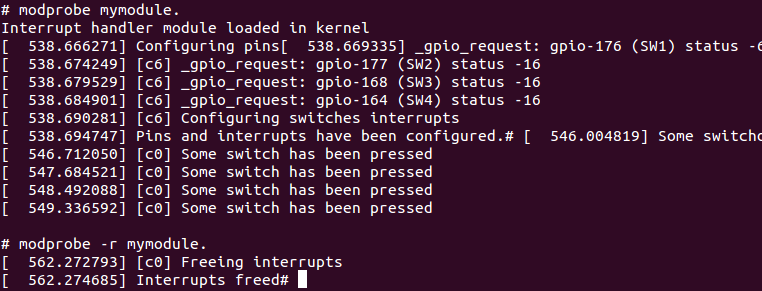
\includegraphics[width=14cm]{img/interrupt_success.png}
		\caption{Affichage du chargement du module, des pressions sur les boutons et de la suppression du module}
		\label{ser1ex9}
	\end{center}
\end{figure}
